\section{O Método de Diferenças Finitas (MDF)}

Uma equação diferencial parcial, que geralmente é considerada em um domínio
contínuo, pode ser discretizada. Isso é feito para que a equação possa ser
representada e resolvida computacionalmente.

No caso do Método de Diferenças	Finitas para esse trabalho, basta
transcrever cada termo da equação para o equivalente na fórmula de
diferenças finitas nas derivações de segundo grau. Podemos
ver um exemplo disso na Equação \ref{eq:stencil1D}, para o caso da parte
espacial em $x$ da equação.
\begin{equation}
	\dfrac{\partial^2 u}{\partial x^2} \xrightarrow{} \dfrac{u_{i-1,j,k} -
		2u_{i,j,k} + u_{i+1,j,k}}{\Delta x^2}
	\label{eq:stencil1D}
\end{equation}

Para entender o que
significa o índice $i$ visto na Equação acima pode-se seguir uma analogia:
suponhamos um \textit{array} com mais que três posições. A posição $i$ seria
qualquer posição intermediária, $i-1$ a antecessora e a $i+1$ sucessora. Tal
estrutura é chamada de \textbf{estêncil}. O mesmo vale para os índices
$j$ e $k$, mas para um \textit{array} com três dimensões. Podemos ver
uma alegoria dessa analogia na Figura \ref{fig:stencil1D}.
\begin{figure}[H]
	\centering
	\label{fig:stencil1D}
	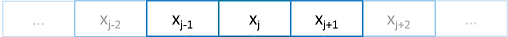
\includegraphics[scale=.5, width=\textwidth]{chapters/chp2/images/1d-stencil.png}
	\caption{\textit{Stencil} unidimensional \cite{image:1d-stencil}}
\end{figure}

No caso desse trabalho, para a simulação da propagação de ondas em um
meio bidimensional ao longo do tempo, teremos que usar três estênceis
(os dois restantes podem ser vistos nas Equações
\ref{eq:stencils3D-1} e \ref{eq:stencils3D-2}), dois para as dimensões
espaciais e um para a temporal. Para tal,
podemos utilizar outra analogia: um \textit{array} tridimensional, onde cada
plano de posições no espaço é um instante no tempo.
\begin{align}
	\dfrac{\partial^2 u}{\partial y^2} & \xrightarrow{} \dfrac{u_{i,j-1,k} - 2u_{i,j,k} +
		u_{i,j+1,k}}{\Delta y^2}
	\label{eq:stencils3D-1}
	\\
	\dfrac{\partial^2 u}{\partial t^2} & \xrightarrow{} \dfrac{u_{i,j,k-1} - 2u_{i,j,k} +
		u_{i,j,k+1}}{\Delta t^2}
	\label{eq:stencils3D-2}
\end{align}

Contudo, até então, não falamos sobre o Método de Diferenças Finitas
em si. Trata-se de uma sequência de iterações que marcham em função de
alguma variável. No caso desse trabalho, o avanço se dá no tempo. Essa marcha
no tempo quer dizer que o valor para um ponto no espaço no próximo instante de
tempo será calculado com base nos valores para pontos no espaço em instantes
anteriores. Vamos ser explícitos. Temos que a equação \ref{eq:waveEq} traduzida
nas fórmulas vistas nas Equações
\ref{eq:stencil1D}, \ref{eq:stencils3D-1} e \ref{eq:stencils3D-2} se dá por
\begin{equation}
	\begin{split}
		\dfrac{u_{i,j,k-1} - 2u_{i,j,k} + u_{i,j,k+1}}{\Delta t^2} = \dfrac{1}{v^2}(\dfrac{u_{i-1,j,k} - 2u_{i,j,k} + u_{i+1,j,k}}{\Delta x^2} \\+ \dfrac{u_{i,j-1,k} - 2u_{i,j,k} + u_{i,j+1,k}}{\Delta y^2}) + f(x, y, t)
	\end{split}
\end{equation}
onde $u_{k+1}$ é o ponto com valor a ser calculado para o próximo
instante. Logo, ele precisa ser isolado, o que é mostrado na equação
\ref{eq:timeMarching}
\begin{equation}
	\begin{split}
		\label{eq:timeMarching}
		u_{i, j,k+1} = \dfrac{\Delta t^2}{v^2} \left(\dfrac{u_{i-1,j,k} - 2u_{i,j,k} + u_{i+1,j,k}}{\Delta x^2} + \dfrac{u_{i,j-1k} - 2u_{i,j,k} + u_{i,j+1,k}}{\Delta y^2}\right) + \\\Delta t^2f(x, y, t) - u_{i,j,k-1} + 2u_{i,j,k}
	\end{split}
\end{equation}